
\chapter{Retropropagación en redes neuronales rotalmente conectadas} \label{backprop_fully_apendice}

En esta sección, se analizará en profundidad el cálculo del gradiente de la pérdida con respecto a cada parámetro entrenable de una red totalmente conectada, así como con respecto a la entrada y salida de cada capa. Primero, se presentarán los cálculos para ejemplos concretos, y, una vez comprendidas las bases, se mostrará cómo aplicarlos a cualquier tipo de red totalmente conectada.

\section{Retropropagación con 1 capa oculta \cite{NN_backpropagation} \cite{NN_backprop_2} \label{backprop_1_capa}}

En esta sección, se tratará de calcular el gradiente de la pérdida con respecto a cada parámetro de la red totalmente conectada, mostrada en la Figura \ref{fig:nn_1_capa}. Para no repetir cálculos, en esta y secciones posteriores, no se volverá a calcular la retropropagación a través de la capa SoftMax, pues los cálculos son siempre los mismos por ser la última capa de la arquitectura.

\begin{figure}[H]
	\centering
	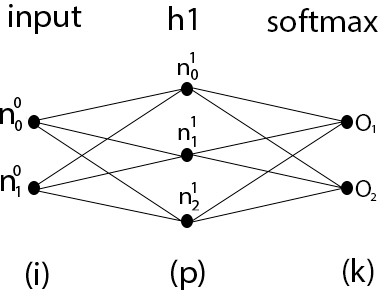
\includegraphics[scale=0.35]{imagenes/nn_1_capa.jpg}  
	\caption{Red Neuronal totalmente conectada con 1 capa oculta}
	\label{fig:nn_1_capa}
\end{figure}

La Figura \ref{fig:nn_1_capa} se compone de 'puntos' interconectados mediante líneas, representando estos neuronas y pesos que las conectan respectivamente. Cada punto corresponde a una neurona, y cada línea a un peso. \\
La Figura \ref{fig:nn_1_capa} presenta 3 capas (input, h1, softmax), que corresponden a la capa de entrada, la capa oculta $h_1$, y la capa de salida, respectivamente. El superíndice indica la capa a la que pertenece una neurona o peso, mientras que el subíndice indica el número del mismo en su respectiva capa. En el caso de los pesos, se requieren 2 subíndices para identificar a cada uno, (cada peso une 2 neuronas). \\
De esta manera, la capa de entrada se compone de 2 neuronas ($n^{0}_0$ y $n^{0}_1$), la capa oculta $h_1$ tiene 3 neuronas ($n^1_{0}$, $n^1_{1}$, y $n^1_{2}$), y el peso $W^{i}_{jk}$ referencia al peso que une las neuronas $n^{i}_j$ y $n^{i+1}_k$.\\
De forma adicional, se recuerda que $Z_i$ representa la entrada $i$ de la capa SoftMax, y, $O_i$, su salida.  

\subsection{Capa SoftMax}

\begin{figure}[H]
	\centering
	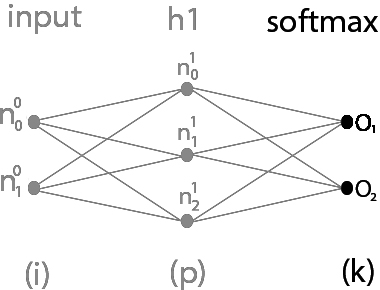
\includegraphics[scale=0.35]{imagenes/nn_1_capa_output.jpg}  
	\caption{Retropropagación en la capa softmax}
	\label{fig:nn_1_capa_output}
\end{figure}

Sea la neurona $n^i_j$, se define como $a^i_j$ el valor de dicha neurona antes de aplicar sobre ella su función de activación asociada, y, $z^i_j$, el obtenido tras aplicarla. 

Tal y como se calculó previamente, el gradiente de la función de pérdida con respecto a cada $Z_i$ viene dado por la fórmula \ref{gradiente_softmax}.


\subsection{Pesos capas h1-SoftMax}

\begin{figure}[H]
	\centering
	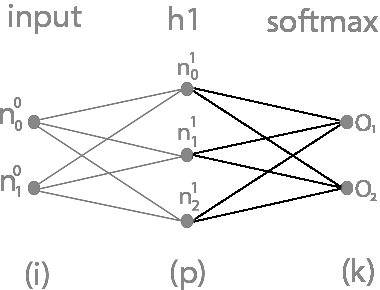
\includegraphics[scale=0.35]{imagenes/nn_1_capa_pesos_h1_output.jpg}  
	\caption{Retropropagación con respecto a pesos entre la capa oculta y la capa SoftMax}
	\label{fig:nn_1_pesos_h1_output}
\end{figure}

Una vez obtenido el gradiente hasta la entrada de la capa softmax, se puede calcular el gradiente con respecto a cada peso $W^1_{pk}$, pues se encuentra conectado a esta desde la capa anterior. Es decir, para cada $n^1_p\in h_1$, se calcula $\frac{dE(x)}{dW^1_{pk}}$. Usando la regla de la cadena, equivale a realizar lo ilustrado en las fórmulas \ref{grad_w1pk_1} y \ref{grad_w1pk_2}.

\begin{gather}
	\frac{\partial Z_k}{\partial W^1_{pk}} = \frac{\partial (z^1_p   W^1 _{pk}+ b^2_k)}{\partial W^1_{pk }} = z^1_p
	\label{grad_w1pk_1}
\end{gather}

\begin{gather}
	\frac{\partial E(x)}{\partial W^1_{pk }} =  gradiente\_Z_k   \frac{\partial Z_k}{\partial W^1_{pk }} = gradiente\_Z_k   z^1_p
	\label{grad_w1pk_2}
\end{gather}

\subsection{Sesgos capa softmax}

Del mismo modo, se calcula el gradiente de la pérdida con respecto a cada sesgo de las neuronas de la capa softmax, tal y como se muestra en las fórmulas \ref{grad_b_h1_1}, \ref{grad_b_h1_2} y \ref{grad_b_h1_3}.

\begin{gather}
	\frac{\partial E}{\partial b^2_k} = \frac{\partial E}{\partial Z_k}   \frac{\partial Z_k}{b^2_k} \label{grad_b_h1_1} \\
	\frac{\partial Z_k }{\partial b^2_k } = \frac{\partial ([\sum_{c=1}^{P} z^1_c   W^1_{pk}] + b^2_k) }{\partial b^2_k } = 1 \label{grad_b_h1_2} \\
	\frac{\partial E}{\partial b^2_k} = gradiente\_Z_k \label{grad_b_h1_3}
\end{gather}

\subsection{Capa oculta h1}

\begin{figure}[H]
	\centering
	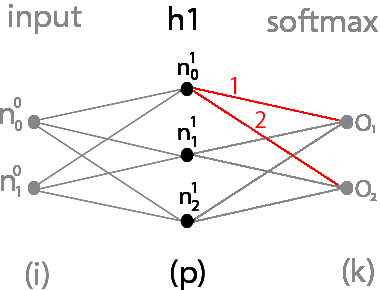
\includegraphics[scale=0.35]{imagenes/nn_caminos_posibles.jpg}  
	\caption{Imagen de los 'caminos' desde la capa softmax hasta la neurona $n^1_0$}
	\label{nn_caminos_posibles}
\end{figure}

En la figura \ref{nn_caminos_posibles}, se muestra como hay más de un 'camino' desde la capa softmax hasta $n^1_p$. Por lo tanto, para obtener el gradiente de la pérdida con respecto a $n^1_p$, es necesario calcular la suma de todos los 'caminos' hacia este, tal y como se presenta en las fórmulas \ref{E_total_a1p} y \ref{deriv_Zk_z1p}. \\

\begin{gather}
	\frac{\partial E_{total}}{\partial a^1_p} = \sum_{k=1}^K \frac{\partial E_k}{\partial a^1_p} = \sum_{k=1}^K  gradiente\_Z_k   \frac{\partial Z_k}{\partial z^1_p}   \frac{\partial z^1_p}{\partial a^1_p}
	\label{E_total_a1p}
\end{gather}

\begin{gather}
	\frac{\partial Z_k}{\partial z^1_p} = \frac{\partial( [\sum_{c=1}^{P} z^1_c   W^1_{ck}] + b^2_k)}{\partial z^1_p} = W^1_{pk}
	\label{deriv_Zk_z1p}
\end{gather}

Para calcular dichos gradientes, se requiere calcular $\frac{\partial z^1_p}{\partial a^1_p}$. Como se mencionó anteriormente, ``a'', se refiere al valor de una neurona antes de aplicar su función de activación asociada, y, ``z'', al valor obtenido tras su aplicación. Por lo tanto, para calcular $\frac{\partial z^1_p}{\partial a^1_p}$, se requiere conocer dicha función de activación.

\begin{figure}[H]
	\centering
	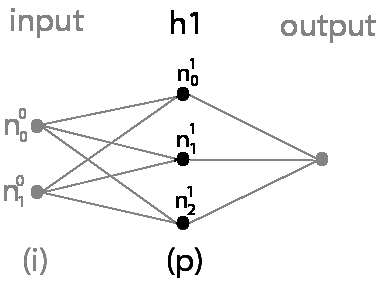
\includegraphics[scale=0.35]{imagenes/nn_1_capa_h1.jpg}  
	\caption{Retropropagación con respecto a neuronas de la capa oculta h1}
	\label{fig:nn_1_capa_h1}
\end{figure}

En este ejemplo, en la capa oculta h1 se emplea la función de activación sigmoide, y su derivada viene dada por las fórmulas \ref{grad_sig_1} y \ref{grad_sig_2}. 

\begin{gather}
	sigmoide(x) = \frac{1}{1+e^{-x}} \label{grad_sig_1} \\
	sigmoide'(x) = \frac{sigmoide(x)}{1-sigmoide(x)} \label{grad_sig_2}
\end{gather}

De este modo, ahora sí se puede calcular $\frac{\partial z^1_p}{\partial a^1_p}$, y se muestra en la fórmula \ref{deriv_z1p_a1p}.

\begin{gather}
	\frac{\partial z^1_ p}{\partial a^1_p} = \frac{\partial sigmoide(a^1_p)}{\partial a^1_p} = sigmoide(a^1_p) (1-sigmoide(a^1_p))
	\label{deriv_z1p_a1p}
\end{gather}

Así, se retoma la fórmula \ref{E_total_a1p} mediante la aplicación de \ref{deriv_Zk_z1p} y \ref{deriv_z1p_a1p}, y se obtiene \ref{grad_E_a1p}.

\begin{gather}
	\frac{\partial E_{total}}{\partial a^1_p} = \sum_{k=1}^K  gradiente\_Z_k   W^1_{pk}   sigmoide(a^1_p) (1-sigmoide(a^1_p)) \label{grad_E_a1p} \\
	\frac{\partial E_{total}}{\partial a^1_p} = gradiente\_h1_p \notag
\end{gather}

\subsection{Pesos capas entrada-h1}

Una vez realizada la retropropagación hasta las neuronas de entrada de la capa oculta h1, se puede continuar con el proceso hacia la capa anterior, es decir, la capa de entrada.

\begin{figure}[H]
	\centering
	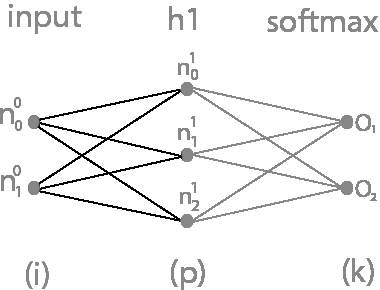
\includegraphics[scale=0.35]{imagenes/nn_1_capa_pesos_input_h1.jpg}  
	\caption{Retropropagación con respecto a los pesos entre la capa de entrada y la capa oculta h1}
	\label{fig:nn_1_pesos_input_h1}
\end{figure}


\begin{gather}
	\frac{\partial a^1_p }{\partial W^0_{ip} } = \frac{\partial [\sum_{c=1}^{I} z^0_c   W^0_{cp}] + b^1_p)}{\partial W^0_{ip} } = z^0_i \label{grad_w0ip_1} \\
	\frac{\partial E}{\partial W^0_{ip}} = \frac{\partial E_{total} }{\partial a^1_p }   \frac{\partial a^1_p}{W^0_{ip}} \label{grad_w0ip_2} \\
	\frac{\partial E(x) }{\partial W^0_{ip} } = gradiente\_h1_p   \frac{\partial a^1_p }{\partial W^0_{ip} } = gradiente\_h1_p   z^0_i 
	\label{grad_w0ip_3}
\end{gather}

De manera similar a como se calcularon los gradientes de la pérdida con respecto a los pesos entre la capa oculta $h_1$ y la capa softmax, se calcula el gradiente de la pérdida con respecto a los pesos entre la capa de entrada y la capa oculta h1. Este proceso se detalla en las fórmulas \ref{grad_w0ip_1}, \ref{grad_w0ip_2}, y \ref{grad_w0ip_3}.

\subsection{Sesgos capa h1}

\begin{gather}
	\frac{\partial E}{\partial b^1_p} = \frac{\partial E_{total} }{\partial a^1_p }   \frac{\partial a^1_p}{b^1_p} \label{grad_b1p_1} \\
	\frac{\partial a^1_p }{\partial b^1_p } = \frac{\partial ([\sum_{c=1}^{I} z^0_c   W^0_{ip}] + b^1_p) }{\partial b^1_p } = 1 \label{grad_b1p_2} \\
	\frac{\partial E}{\partial b^1_p} = gradiente\_h1_p
	\label{grad_b1p_3}
\end{gather}

De manera similar, las figuras \ref{grad_b1p_1}, \ref{grad_b1p_2}, y \ref{grad_b1p_3} ilustran el cálculo del gradiente con respecto a los sesgos de la capa oculta h1.

\subsection{Capa de entrada}

\begin{figure}[H]
	\centering
	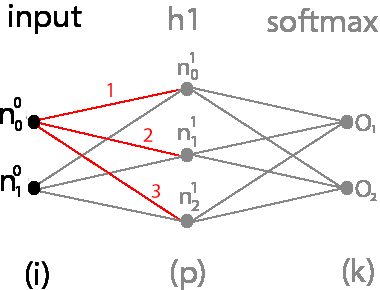
\includegraphics[scale=0.35]{imagenes/nn_caminos_posibles_input.jpg}  
	\caption{Imagen de los 'caminos' desde la capa oculta h1 hasta $n^0_0$}
	\label{nn_caminos_posibles_input}
\end{figure}

Por último, en esta sección se calcula el gradiente con respecto a las neuronas de entrada de la capa de entrada. Aunque, en general, no sería necesario calcular estos gradientes, dado que el objetivo es construir una red neuronal convolucional (CNN), es imprescindible hacerlo. Esto se debe a que la red totalmente conectada estará integrada con capas convolucionales y de agrupación máxima, por lo que es necesario calcular estos gradientes para poder continuar con el proceso de retropropagación en las capas anteriores a esta.

\begin{gather}
	\frac{\partial E_{total}}{\partial a^0_i} = \sum_{p=1}^P \frac{\partial E_{total}}{\partial a^1_p}   \frac{\partial a^1_p}{\partial z^0_i}   \frac{\partial z^0_i}{\partial a^0_i} \notag \\
	\frac{\partial a^1_p }{\partial z^0_i } = \frac{\partial ([\sum_{c=1}^{I} z^0_c   W^0_{ip}] + b^1_p) }{\partial z^0_i } = W^0_{ip} \label{grad_a_2}
\end{gather}

\begin{figure}[H]
	\centering
	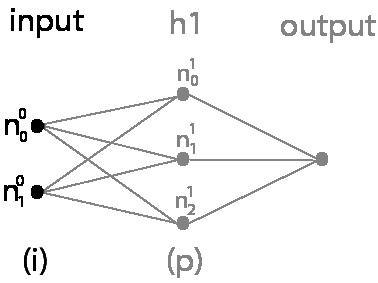
\includegraphics[scale=0.35]{imagenes/nn_1_capa_input.jpg}  
	\caption{Retropropagación en la capa input}
	\label{fig:nn_1_capa_input}
\end{figure}

Como la capa input no presenta ninguna función de activación asociada, se tiene que $z^0_i$ es igual $a^0_i$. \\

\begin{gather}
	\frac{\partial z^0_i }{\partial a^0_i } = 1 \\
	\frac{\partial E_{total}}{\partial a^0_i} = \sum_{p=1}^{P} gradiente\_h1_p
\end{gather}

\section{Retropropagación con 2 capas ocultas}

\begin{figure}[H]
	\centering
	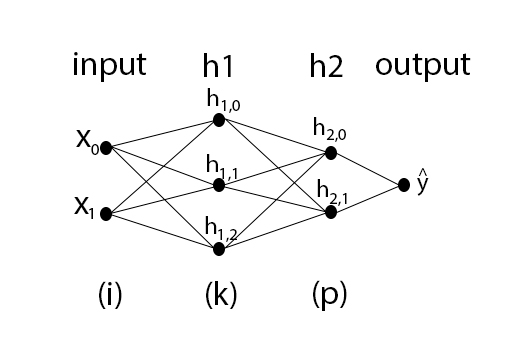
\includegraphics[scale=0.35]{imagenes/nn_2_capas.jpg}  
	\caption{Red Neuronal totalmente conectada con 2 capas ocultas}
	\label{fig:nn_2_capas}
\end{figure}

A diferencia del apartado anterior, en este caso se utiliza una red totalmente conectada con 2 capas ocultas (h1 y h2), tal y como se muestra en la Figura \ref{fig:nn_2_capas}. \\

\subsection{Capa SoftMax}

\begin{figure}[H]
	\centering
	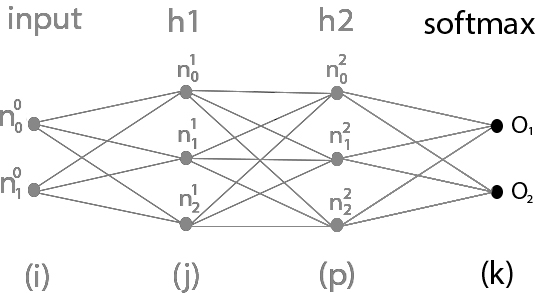
\includegraphics[scale=0.35]{imagenes/nn_2_capa_output.jpg}  
	\caption{Retropropagación en la capa softmax}
\end{figure}

De manera similar a los casos anteriores, el gradiente de la función de pérdida con respecto a cada $Z_i$, se determina mediante la fórmula \ref{gradiente_softmax}. En consecuencia, no se repetirá el cálculo. \\

\subsection{Pesos capas h2-SoftMax}

\begin{figure}[H]
	\centering
	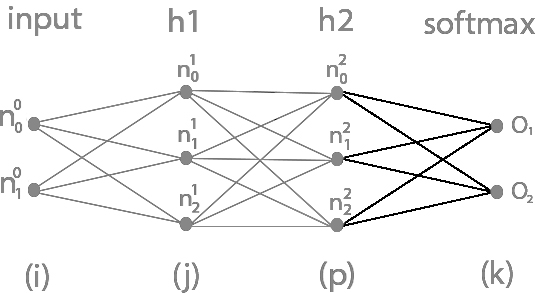
\includegraphics[scale=0.35]{imagenes/nn_2_capa_pesos_h2_output.jpg}  
	\caption{Retropropagación respecto a los pesos entre la capa oculta h2 y la capa SoftMax}
	\label{fig:nn_2_capa_pesos_h2_output}
\end{figure}

Se lleva a cabo el cálculo del gradiente de la función de pérdida con respecto a cada peso $W^2_{pk}$ que conecta las neuronas de la capa oculta h2 con las de la capa softmax (véase la figura \ref{fig:nn_2_capa_pesos_h2_output}). \\

\begin{gather}
	\frac{\partial Z_k}{\partial W^2_{pk}} = \frac{\partial (z^2_p   W^2 _{pk} + b^3_k)}{\partial W^2_{pk }} = z^2_p 
	\label{grad_w2pk_1}
\end{gather}

\begin{gather}
	\frac{\partial E(x)}{\partial W^2_{pk }} =  gradiente\_Z_k   \frac{\partial Z_k}{\partial W^2_{pk }} = gradiente\_Z_k   z^2_p
	\label{grad_w2pk_2}
\end{gather}

Como era de esperar, las fórmulas \ref{grad_w2pk_1} y \ref{grad_w2pk_2} son prácticamente idénticas a las fórmulas \ref{grad_w1pk_1} y \ref{grad_w1pk_2}, respectivamente, con la única diferencia del superíndice empleado (1 $\neq$ 2). Esto resulta lógico, ya que esta parte del cálculo es también común al apartado anterior.

\subsection{Sesgos capa softmax}

\begin{gather}
	\frac{\partial E}{\partial b^3_k} = \frac{\partial E}{\partial Z_k}   \frac{\partial Z_k}{b^3_k} \label{grad_b_h2_1} \\
	\frac{\partial Z_k }{\partial b^3_k } = \frac{\partial ([\sum_{c=1}^{P} z^2_c   W^2_{pk}] + b^3_k) }{\partial b^3_k } = 1 \label{grad_b_h2_2} \\
	\frac{\partial E}{\partial b^3_k} = gradiente\_Z_k \label{grad_b_h2_3}
\end{gather}

De manera similar, el cálculo del gradiente de la pérdida con respecto a los sesgos de la capa softmax también se mantiene inalterado. Por consiguiente, la única diferencia entre las fórmulas $\{$\ref{grad_b_h2_1}, \ref{grad_b_h2_2}, \ref{grad_b_h2_3}$\}$ y $\{$\ref{grad_b_h1_1}, \ref{grad_b_h1_2}, \ref{grad_b_h1_3}$\}$ radica en los superíndices utilizados.

\subsection{Capa oculta h2}

\begin{figure}[H]
	\centering
	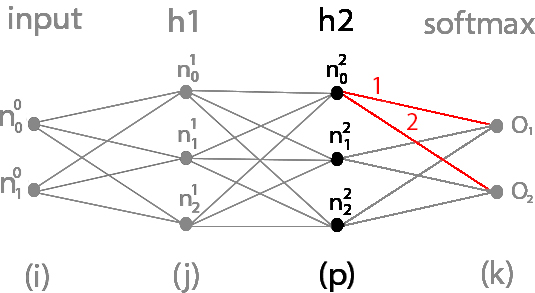
\includegraphics[scale=0.35]{imagenes/nn_h2_caminos_posibles.jpg}  
	\caption{Imagen de los 'caminos' desde la capa softmax hasta $n^2_0$}
	\label{nn_h2_caminos_posibles}
\end{figure}

Tal y como se comentó anteriormente, existen mútiples 'caminos' desde la capa softmax hasta $n^2_p$. Por lo tanto, para obtener el gradiente de la pérdida con respecto a cada $n^2_p$, es necesario calcular la suma de todos ellos, tal y como se detalla en las fórmulas \ref{E_total_a2p} y \ref{deriv_Zk_z2p}. \\

\begin{gather}
	\frac{\partial E_{total}}{\partial a^2_p} = \sum_{k=1}^K \frac{\partial E_k}{\partial a^2_p} = \sum_{k=1}^K  gradiente\_Z_k   \frac{\partial Z_k}{\partial z^2_p}   \frac{\partial z^2_p}{\partial a^2_p}
	\label{E_total_a2p}
\end{gather}

\begin{gather}
	\frac{\partial Z_k}{\partial z^2_p} = \frac{\partial( [\sum_{c=1}^{P} z^2_c   W^2_{ck}] + b^3_k)}{\partial z^2_p} = W^2_{pk}
	\label{deriv_Zk_z2p}
\end{gather}

\begin{figure}[H]
	\centering
	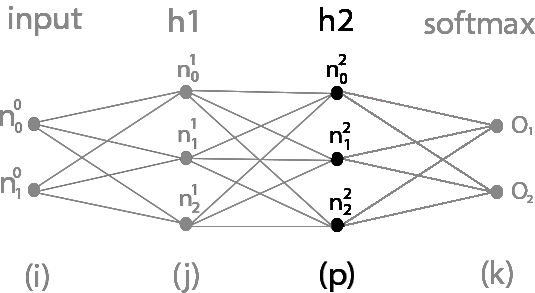
\includegraphics[scale=0.35]{imagenes/nn_2_capa_h2.jpg}  
	\caption{Retropropagación en la capa oculta h2}
	\label{fig:nn_2_capa_h2}
\end{figure}

Dado que coincide con el ejemplo anterior, en la última capa oculta (en este caso, h2), se utiliza nuevamente la función de activación sigmoide. Por lo tanto, se reitera la derivada de esta función en las fórmulas \ref{grad_sig_h2_1} y \ref{grad_sig_h2_2} para facilitar la comprensión del lector.

\begin{gather}
	sigmoide(x) = \frac{1}{1+e^{-x}} \label{grad_sig_h2_1} \\
	sigmoide'(x) = \frac{sigmoide(x)}{1-sigmoide(x)} \label{grad_sig_h2_2}
\end{gather}


Empleando la derivada de sigmoide, se obtiene la fórmula \ref{deriv_z2p_a2p}.

\begin{gather}
	\frac{\partial z^2_ p}{\partial a^2_p} = \frac{\partial sigmoide(a^2_p)}{\partial a^2_p} = sigmoide(a^2_p) (1-sigmoide(a^2_p))
	\label{deriv_z2p_a2p}
\end{gather}

A continuación, se retoma la fórmula \ref{E_total_a2p} mediante la aplicación de \ref{deriv_Zk_z2p} y \ref{deriv_z2p_a2p} para obtener \ref{grad_E_a2p}.

\begin{gather}
	\frac{\partial E_{total}}{\partial a^2_p} = \sum_{k=1}^K  gradiente\_Z_k   W^2_{pk}   sigmoide(a^2_p) (1-sigmoide(a^2_p)) \label{grad_E_a2p} \\
	\frac{\partial E_{total}}{\partial a^2_p} = gradiente\_h2_p \notag
\end{gather}

Una vez más, la fórmula obtenida (\ref{grad_E_a2p}) coindice con la calculada previamente (\ref{grad_E_a1p}), salvo por los superíndices empleados. \\

\subsection{Pesos capas h1-h2}

\begin{figure}[H]
	\centering
	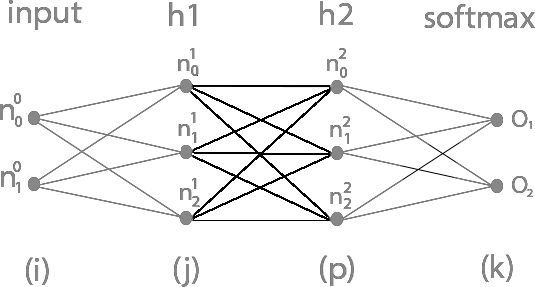
\includegraphics[scale=0.35]{imagenes/nn_2_capa_pesos_h1_h2.jpg}  
	\caption{Retropropagación respecto a los pesos entre las capas ocultas h1 y h2}
	\label{fig:nn_2_pesos_h1_h2}
\end{figure}


\begin{gather}
	\frac{\partial a^2_p }{\partial W^1_{jp} } = \frac{\partial [\sum_{c=1}^{J} z^1_c   W^1_{cp}] + b^2_p)}{\partial W^1_{jp} } = z^1_j \notag \\
	\frac{\partial E}{\partial W^1_{jp}} = \frac{\partial E_{total} }{\partial a^2_p }   \frac{\partial a^2_p}{W^1_{jp}} \notag \\
	\frac{\partial E(x) }{\partial W^1_{jp} } = gradiente\_h2_p   \frac{\partial a^2_p }{\partial W^1_{jp} } = gradiente\_h2_p   z^1_j 
	\label{grad_w1jp}
\end{gather}

Dado que esta parte también es común al caso anterior, la fórmula \ref{grad_w1jp} coincide nuevamente con la fórmula \ref{grad_w0ip_3}.


\subsection{Sesgos capa h2}

\begin{gather}
	\frac{\partial E}{\partial b^2_p} = \frac{\partial E_{total} }{\partial a^2_p }   \frac{\partial a^2_p}{b^2_p} \notag \\
	\frac{\partial a^2_p }{\partial b^2_p } = \frac{\partial ([\sum_{c=1}^{J} z^1_c   W^1_{jp}] + b^2_p) }{\partial b^2_p } = 1 \notag \\
	\frac{\partial E}{\partial b^2_p} = gradiente\_h2_p
	\label{grad_b2p}
\end{gather}

Una vez más, la fórmula \ref{grad_b2p} coincide con \ref{grad_b1p_3}. Es fundamental reconocer las partes comunes entre ambos casos, ya que esto facilita la generalización del modelo y la automatización de los cálculos correspondientes.

\subsection{Capa oculta h1}

\begin{figure}[H]
	\centering
	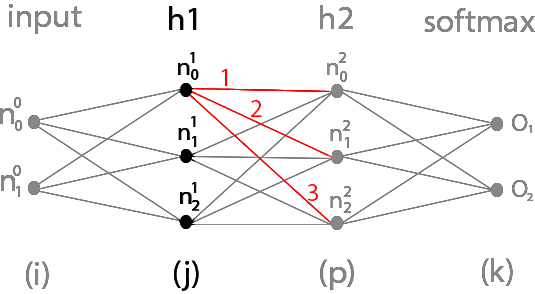
\includegraphics[scale=0.35]{imagenes/nn_h1_caminos_posibles.jpg}  
	\caption{'Caminos' desde la capa softmax hasta $n^1_0$}
	\label{nn_h1_caminos_posibles}
\end{figure}

De manera similar a lo realizado en la capa h2, se calcula la suma de todos los 'caminos' hacia cada neurona $n^1_j$. \\

\begin{gather}
	\frac{\partial E_{total}}{\partial a^1_j} = \sum_{k=1}^K \frac{\partial E_k}{\partial a^1_j} = \sum_{p=1}^P  gradiente\_h2_p   \frac{\partial a^2_p}{\partial z^1_j}   \frac{\partial z^1_j}{\partial a^1_j} \notag \\
	\frac{\partial a^2_p}{\partial z^1_j} = \frac{\partial( [\sum_{c=1}^{J} z^1_c   W^1_{cp}] + b^2_p)}{\partial z^1_j} = W^1_{jp} \notag
\end{gather}

Como era de esperar, se calcula el gradiente con respecto a cada neurona de la capa h1 considerando cada `camino' del gradiente proveniente la capa siguiente (h2).

\begin{figure}[H]
	\centering
	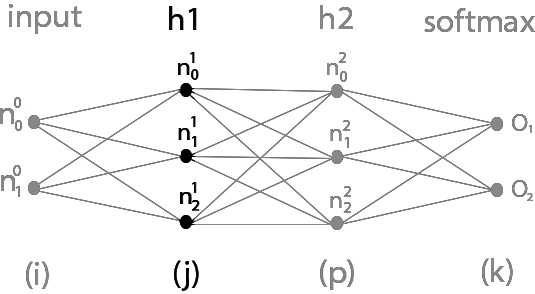
\includegraphics[scale=0.35]{imagenes/nn_2_capa_h1.jpg}  
	\caption{Retropropagación en la capa oculta h1}
\end{figure}

En este caso, en la capa oculta h1 se utiliza la función de activación ReLU, cuya derivada viene dada por la fórmula \ref{deriv_relu}. 

\begin{gather}
	ReLU(x) = max(0, x) \label{relu} \\
	ReLU'(x) = 1\ si\ x>0,\ 0\ en\ caso\ contrario
	\label{deriv_relu}
\end{gather}

La derivada la función de activación ReLU (fórmula \ref{relu}), se emplea para obtener el gradiente $\frac{\partial z^1_ j}{\partial a^1_j}$, y para continuar con la retropropagación a través de la capa, tal y como se detalla en las fórmulas (\ref{grad_E_a1j_1}, \ref{grad_E_a1j_2}, y \ref{grad_E_a1j_3}).


\begin{gather}
	\frac{\partial z^1_ j}{\partial a^1_j} = 1\ si\ x>0,\ 0\ en\ caso\ contrario \label{grad_E_a1j_1} \\
	\frac{\partial E_{total}}{\partial a^1_j} = \sum_{p=1}^P  gradiente\_h2_p   W^1_{jp}   ReLU'(a^1_j) \label{grad_E_a1j_2} \\
	\frac{\partial E_{total}}{\partial a^1_j} = gradiente\_h1_j
	\label{grad_E_a1j_3}
\end{gather}

Una vez más, el proceso para obtener de la fórmula \ref{grad_E_a1j_2} es muy similar al utilizado en casos anteriores, a pesar de que pueda parecer relativamente nueva en comparación con la sección anterior. \\


\subsection{Pesos capa input-h1}

\begin{figure}[H]
	\centering
	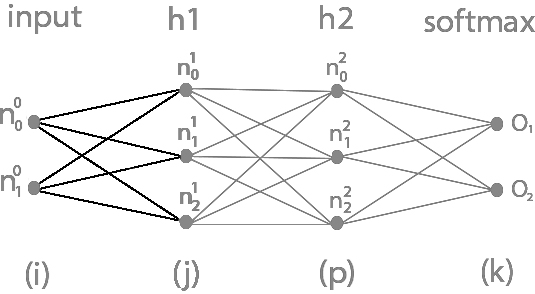
\includegraphics[scale=0.35]{imagenes/nn_2_capa_pesos_input_h1.jpg}  
	\caption{Retropropagación respecto a los pesos entre la capa de entrada y la capa oculta h1}
	\label{fig:nn_2_pesos_input_h1}
\end{figure}


\begin{gather}
	\frac{\partial a^1_j }{\partial W^0_{ij} } = \frac{\partial ([\sum_{c=1}^{I} z^0_c   W^0_{cj}] + b^1_j)}{\partial W^0_{ij} } = z^0_i \label{grad_w0ip_h2_1} \\
	\frac{\partial E}{\partial W^0_{ij}} = \frac{\partial E_{total} }{\partial a^1_j }   \frac{\partial a^1_j}{W^0_{ij}} \label{grad_w0ip_h2_2} \\
	\frac{\partial E(x) }{\partial W^0_{ij} } = gradiente\_h1_j   \frac{\partial a^1_j }{\partial W^0_{ij} } = gradiente\_h1_j   z^0_i \label{grad_w0ip_h2_3}
\end{gather}

Aquí se observa que las fórmulas $\{$\ref{grad_w0ip_h2_1}, \ref{grad_w0ip_h2_2}, \ref{grad_w0ip_h2_3} $\}$ son idénticas a $\{$\ref{grad_w0ip_1}, \ref{grad_w0ip_2}, \ref{grad_w0ip_3} $\}$, excepto por el subíndice empleado (j $\neq$ p). Aunque los valores analíticos puedan diferir debido a las diferencias en las arquitecturas, la notación utilizada se ha diseñado para facilitar la visualización y comprensión de la capacidad de automatización en las capas totalmente conectadas.

\subsection{Sesgos capa h1}

\begin{gather}
	\frac{\partial E}{\partial b^1_j} = \frac{\partial E_{total} }{\partial a^1_j }   \frac{\partial a^1_j}{b^1_j} \label{grad_b1j_h2_1} \\
	\frac{\partial a^1_j }{\partial b^1_j } = \frac{\partial ([\sum_{c=1}^{I} z^0_c   W^0_{ij}] + b^1_j) }{\partial b^1_j } = 1 \label{grad_b1j_h2_2} \\
	\frac{\partial E}{\partial b^1_j} = gradiente\_h1_j
	\label{grad_b1j_h2_3}
\end{gather}

De este modo, las fórmulas $\{$\ref{grad_b1j_h2_1}, \ref{grad_b1j_h2_2}, \ref{grad_b1j_h2_3} $\}$ y $\{$\ref{grad_b1p_1}, \ref{grad_b1p_2}, \ref{grad_b1p_3} $\}$ coinciden en todo los aspectos, excepto en el subíndice (j $\neq$ p).

\subsection{Capa input}

\begin{figure}[H]
	\centering
	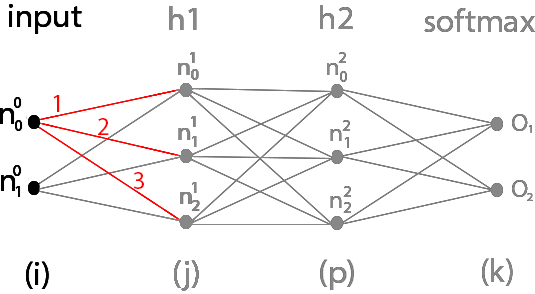
\includegraphics[scale=0.35]{imagenes/nn_2_capas_caminos_posibles_input.jpg}  
	\caption{'Caminos' desde la capa oculta h1 hasta $n^0_0$}
	\label{nn_2_capas_caminos_posibles_input}
\end{figure}

\begin{gather}
	\frac{\partial E_{total}}{\partial a^0_i} = \sum_{j=1}^J \frac{\partial E_{total}}{\partial a^1_j}   \frac{\partial a^1_j}{\partial z^0_i}   \frac{\partial z^0_i}{\partial a^0_i} \label{grad_a_h2_1} \\
	\frac{\partial a^1_j }{\partial z^0_i } = \frac{\partial ([\sum_{c=1}^{I} z^0_c   W^0_{ij}] + b^1_j) }{\partial z^0_i } = W^0_{ij} \label{grad_a_h2_2}
\end{gather}

Aquí también se observa que, a pesar de las diferencias en los subíndices utilizados, las fórmulas $\{$\ref{grad_a_h2_1}, \ref{grad_a_h2_2} $\}$ y $\{$\ref{grad_a_1}, \ref{grad_a_2}$\}$ son idénticas.

\begin{figure}[H]
	\centering
	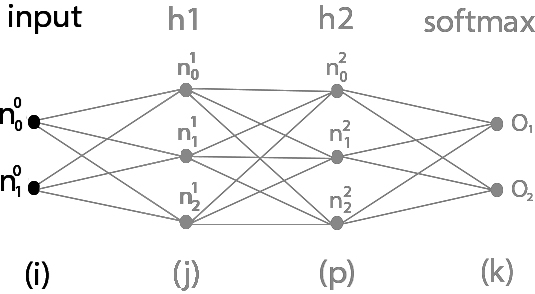
\includegraphics[scale=0.35]{imagenes/nn_2_capa_input.jpg}  
	\caption{Retropropagación en la capa input}
	\label{fig:nn_2_capa_input}
\end{figure}

Dado que la capa de entrada no tiene ninguna función de activación asociada, $z^0_i$ es igual $a^0_i$, al igual que en el caso anterior. \\

\begin{gather}
	\frac{\partial z^0_i }{\partial a^0_i } = 1 \notag \\
	\frac{\partial E_{total}}{\partial a^0_i} = \sum_{p=1}^{P} gradiente\_h1_p \notag
\end{gather}

\section{Conclusiones}
Se definen como capas ocultas ``intermedias'' todas las capas, exceptuando la última de ellas. Tal y como se ha demostrado anteriormente, estas capas comparten la mayoría de los cálculos asociados a la retropropagación. En consecuencia, una red neuronal totalmente conectada puede dividirse en 4 grupos $\{$capa de entrada, capas ocultas intermedias, última capa oculta, capa de salida o capa softmax$\}$. \\
A continuación se realiza el cálculo necesario para la retropropagación de una capa de neuronas \textit{l} específica. Suponemos que la capa \textit{l+1} tiene \textit{Q} neuronas, la capa \textit{l-1} tiene \textit{K} neuronas, y que todas las capas ocultas intermedias usan ReLU como función de activación. \\

\subsection{Gradiente respecto a la entrada de la capa}

\begin{figure}[H]
	\centering
	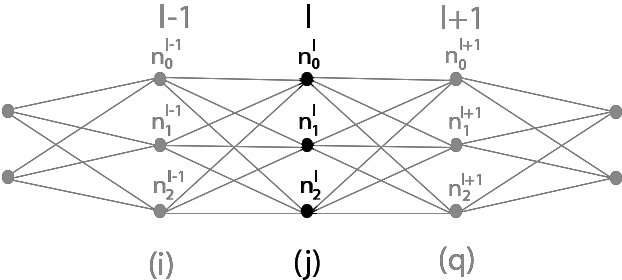
\includegraphics[scale=0.35]{imagenes/conclusion_capa_l.jpg}  
	\caption{Retropropagación en la capa l}
	\label{fig:conclusion_capa_l_apendice}
\end{figure}

\begin{gather}
	\frac{\partial E_{total}}{\partial a^l_j} = \sum_{q=1}^Q \frac{\partial E_{total}}{\partial a^{l+1}_q}   \frac{\partial a^{l+1}_q}{\partial z^l_j}   \frac{\partial z^l_j}{\partial a^l_j} \label{grad_input_l_1} \\
	\frac{\partial a^{l+1}_j }{\partial z^l_j } = \frac{\partial ([\sum_{c=1}^{K} z^l_c   W^l_{ij}] + b^{l+1}_j) }{\partial z^l_j } = W^l_{ij} \label{grad_input_l_2} \\
	\frac{\partial z^l_j}{\partial a^l_j} = ReLU'(a^l_j) \label{grad_input_l_3} \\
	\frac{\partial E_{total}}{\partial a^l_j} = \sum_{q=1}^Q  gradiente\_h_{{l+1}_q}   W^l_{ij}   ReLU'(a^l_j) \label{grad_input_l_4_apendice} \\
	\frac{\partial E_{total}}{\partial a^l_j} = gradiente\_h_{l_j} \label{grad_input_l_5}
\end{gather}

Las fórmulas \ref{grad_input_l_1}, \ref{grad_input_l_2}, \ref{grad_input_l_3},  \ref{grad_input_l_4_apendice}, y \ref{grad_input_l_5}, ilustran el cálculo genérico necesario para obtener el gradiente de la pérdida con respecto a la entrada de una capa oculta intermedia \textit{l}.

\subsection{Gradiente respecto a los pesos}

\begin{figure}[H]
	\centering
	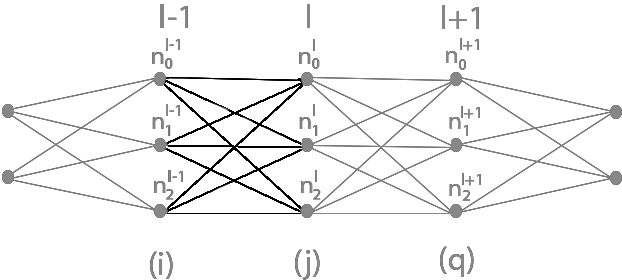
\includegraphics[scale=0.35]{imagenes/conclusion_pesos.jpg}  
	\caption{Retropropagación respecto a los pesos entre la capa l-1 y l}
	\label{fig:conclusion_pesos_apendice}
\end{figure}

\begin{gather}
	\frac{\partial E}{\partial W^{l-1}_{ij}} = \frac{\partial E_{total} }{\partial a^l_j }   \frac{\partial a^l_j}{W^{l-1}_{ij}} \label{grad_w_l_1} \\
	\frac{\partial a^l_j }{\partial W^{l-1}_{ij} } = \frac{\partial ([\sum_{c=1}^{K} z^{l-1}_c   W^{l-1}_{cj}] + b^l_j)}{\partial W^{l-1}_{ij} } = z^{l-1}_i \label{grad_w_l_2} \\
	\frac{\partial E(x) }{\partial W^{l-1}_{ij} } = gradiente\_h_{l_j}   \frac{\partial a^l_j }{\partial W^{l-1}_{ij} } = gradiente\_h_{l_j}   z^{l-1}_i \label{grad_w_l_3_apendice}
\end{gather}

Las fórmulas \ref{grad_w_l_1}, \ref{grad_w_l_2}, y \ref{grad_w_l_3_apendice} detallan el cálculo necesario para determinar el gradiente de la pérdida con respecto a los pesos entre las capas ocultas \textit{l} y \textit{l-1}.

\subsection{Gradiente respecto a sesgos}

\begin{gather}
	\frac{\partial E}{\partial b^l_j} = \frac{\partial E_{total} }{\partial a^l_j }   \frac{\partial a^l_j}{b^l_j} \label{grad_b_l_1} \\
	\frac{\partial a^l_j }{\partial b^l_j } = \frac{\partial ([\sum_{c=1}^{K} z^{l-1}_c   W^{l-1}_{ij}] + b^l_j) }{\partial b^l_j } = 1 \label{grad_b_l_2} \\
	\frac{\partial E}{\partial b^l_j} = gradiente\_h_{l_j} \label{grad_b_l_3_apendice}
\end{gather}

Las fórmulas \ref{grad_b_l_1}, \ref{grad_b_l_2}, y \ref{grad_b_l_3_apendice} presentan el cálculo necesario para obtener el gradiente de la pérdida con respecto a los sesgos de la capa oculta \textit{l}.
